\chapter{Lecture 1 - Introduction}
The course is held by external lecturers, Prof.ssa \textit{Daniela Giorgi} and Prof. \textit{Massimiliano Corsini}.\par
The exam is of 2 parts, a visualization \emph{project} agreed upon with lecturers and an \emph{oral} examination on the notions and concepts presented during the course.\par
The \textbf{main objective} of the course is to learn \textit{how to create an appropriate visualization} for the data we have by learning how to transform data into a graphical representation and when to use different kind of visual representations.

\section{Introduction}
In \textit{scientific visualization}, there is a natural relationship between what is represented and its visual representation, whereas in \textit{information visualization}, the relationship is conventional, and it is up to designer to decide on the best representation. \par
The goal is to transform data to make sense out ot it. 
\subsection{Information visualization}
There are different perspectives to view the information visualization, either as applied science or as a technology.\par
Information visualization as an \textbf{applied science} is that a value of a good visualization let us see patterns in data, and therefore the science of pattern perception can provide a basis for design decisions.\par

Information visualization as a \textbf{technology} is a tool for communication for the understanding and the analysis. The functional constraints from the design of a technological object must depend on the task it should help with, and the graphics form should be constrained by the function of the presentation.\par
\subsection{Why information visualization?}
Human are a visual species. The human visual system is very good at identifying and analyzing patterns. Visualizations are like cognitive artifacts, the tools that help humans to think better, like an abacus. \par
Visualization has to do with distributed cognition. Human cognitive system is made of our brain, mind, and sensors, but also of the environment around us, which we use to store and manipulate information.\par
Visualizations enable parallel processing of information, instead of sequential.\par
Explanatory visualizations are tools to present information, communicate data and messages, and explain something to somebody else. They are tools for readers to analyze what is being presented to them, and very often, the output of the exploratory analysis generates new questions.\par
\begin{figure}[htbp]
    \centering
    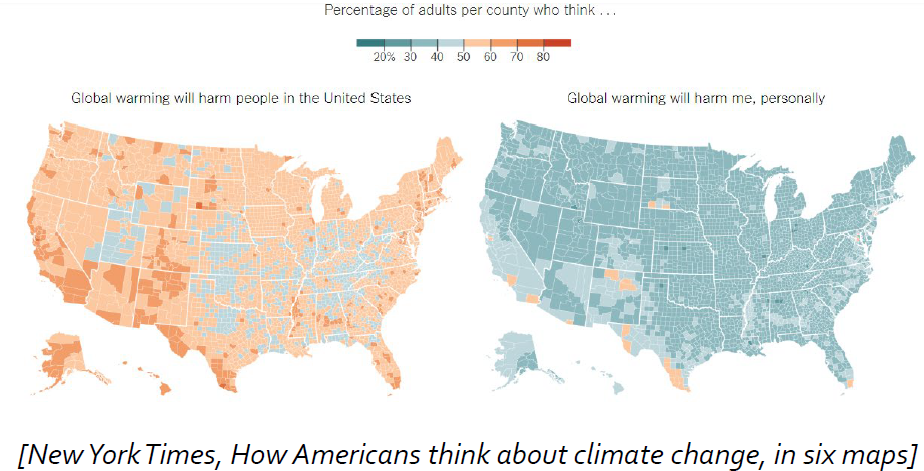
\includegraphics[width=0.5\linewidth]{imgs/lecture1/1.1 explanatory visualization.png}
    \caption{How visualizations convey messages}
    \label{fig:1.1}
\end{figure}
In confirmatory analysis, the reader has an hypothesis, and uses the visualization to see whether their hypothesis is true or not.\par

\subsection{Scientific visualization}
Scientific visualization are computing technique for the generation of interactive visual representations of acquired or simulated spatio-temporal data.\par
Data in ever-increasing sizes makes a graphical approach necessary. The modern process of visualization consists of taking raw data acquired through sensors or produced by some simulation and converting it to a form that is viewable and understandable to humans. \par

They also help us in identifying patterns and interpreting data, either simulated or acquired data. This can find applications in different fields, engineering, medicine, science, biology,...\par


